\documentclass[12pt,twoside,openright]{report}

% Hyperlink references
\usepackage[pdfborder={0 0 0}]{hyperref}
% PGF diagrams
\usepackage{pgf}
\usepackage[utf8]{inputenc}\DeclareUnicodeCharacter{2212}{-}
% Page margins
\usepackage[margin=25mm]{geometry}
% Subfigures
\usepackage{caption}
\usepackage{subcaption}
% Bibliography
\usepackage[style=numeric-comp,sorting=none]{biblatex}
% Images
\usepackage{graphicx}
% Directory tree diagram
\usepackage{dirtree}
% Simple tree diagrams
\usepackage[linguistics]{forest}
\usepackage{adjustbox}
% Algorithms
\usepackage[ruled]{algorithm2e}
% Verbatim++
\usepackage{alltt}
% Text colour
\usepackage{xcolor}
% Better verbatim
\usepackage{fancyvrb}
% TikZ diagrams
\usepackage{tikz}
% UK date
\usepackage[UKenglish]{babel}
\usepackage{csquotes}
% Paragraph spacing
\usepackage{parskip}
% Verbatim in caption
\usepackage{cprotect}
% Aligning equations
\usepackage{amsmath}

\addbibresource{bibliography.bib}

%\renewcommand{\baselinestretch}{1.1}
\raggedbottom

\DeclareRobustCommand{\setmetre}[2]{\ensuremath{
  \vcenter{\offinterlineskip
    \halign{\hfil##\hfil\cr
            $\scriptstyle#1$\cr
            \noalign{\vskip1pt}
            $\scriptstyle#2$\cr}
  }}
}

\definecolor{SPpink}{RGB}{255,20,147}
\definecolor{SPblue}{RGB}{30,144,255}
\definecolor{SPorange}{RGB}{255,140,0}
\definecolor{SPgreen}{RGB}{97,206,60}

\begin{document}

%%%%%%%%%%%%%%%%%%%%%%%%%%%%%%%%%%%%%%%%%%%%%%%%%%%%%%%%%%%%%%%%%%%%%%%%
% Title

\begin{titlepage}
    \pagestyle{empty}

    \rightline{\LARGE \textbf{Max Johnson}}

    \vspace*{60mm}
    \begin{center}
    \Huge
    \textbf{Musical micro-timing for live coding} \\[5mm]
    Computer Science Tripos -- Part II \\[5mm]
    Clare College \\[5mm]
    \today
    \end{center}
\end{titlepage}

%%%%%%%%%%%%%%%%%%%%%%%%%%%%%%%%%%%%%%%%%%%%%%%%%%%%%%%%%%%%%%%%%%%%%%%%
% Proforma, table of contents and list of figures

\pagestyle{plain}

\section*{Declaration}

I, [Name] of [College], being a candidate for Part II of the Computer Science Tripos, hereby declare that this dissertation and the work described in it are my own work, unaided except as may be specified below, and that the dissertation does not contain material that has already been used to any substantial extent for a comparable purpose. I am content for my dissertation to be made available to the students and staff of the University.

\bigskip
\leftline{Signed [signature]}

\medskip
\leftline{Date [date]}


\newpage
\chapter*{Proforma}

{\large
\begin{tabular}{ll}
Name:               & \bf Max Johnson                       \\
College:            & \bf Clare College                     \\
Project Title:      & \bf Musical micro-timing for live coding \\
Examination:        & \bf Computer Science Tripos -- Part II, July 2022  \\
Word Count:         & \bf N/A \\
Project Originator: & Mark Gotham                    \\
Supervisor:         & Mark Gotham                    \\ 
\end{tabular}
}


\section*{Original aims of the project}

TBC


\section*{Work completed}

TBC

\section*{Special difficulties}

TBC
 
\newpage
\tableofcontents

%%%%%%%%%%%%%%%%%%%%%%%%%%%%%%%%%%%%%%%%%%%%%%%%%%%%%%%%%%%%%%%%%%%%%%%

\pagestyle{headings}

\chapter{Introduction}

Text.



\chapter{Preparation}

This chapter will introduce the core theories and background material necessary
to understand the project. I will explain some key concepts in music theory and
live coding and give an overview of the case study musical styles. Next, I will
describe the starting point of this project, expand upon the requirements from
the project proposal, and conclude with an outline of the software engineering
techniques used throughout.



\section{Background} \label{background}


\subsection{Musical metre} \label{metre_background}

A beat is a regularly occurring pulse in music. This is usually the pulse you
might tap your foot along to when listening to a piece of music. Musical metre
describes the ways in which beats are grouped and divided within recurring
cycles. This forms different metrical levels within a hierarchy. Division levels
are ones where the beat has been divided into more, shorter durations. Multiple
levels are ones where the beats are grouped into fewer, longer durations. Figure~\ref{fig:metre_hierarchy_example} 
shows the beat level, and some of the division and multiple levels for a simple \ \setmetre{4}{4} time signature, as well as a tree representation of the metrical hierarchy.
A metre is `simple' if its first division level splits the beat into two, and
`compound' if it splits into three \cite{omt2021}.

\begin{figure}
    \centering
    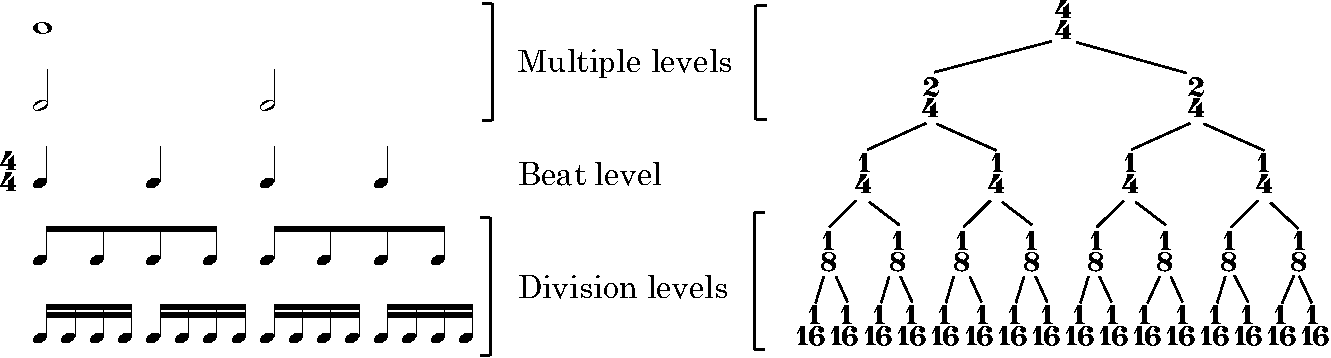
\includegraphics[width=\linewidth]{figures/metre_example.pdf}
    \caption{Example metrical hierarchy for the \setmetre{4}{4} time signature. Left: The hierarchy as notes in traditional Western music notation. Right: The hierarchy as a tree of durations.}
    \label{fig:metre_hierarchy_example}
\end{figure}

Every note in a piece of music occurs at a particular metrical position, but
music performed by humans often deviates from these mechanically even timings
\cite{london2012}. The ways in which these deviations occur contribute significantly
to what we call musical style by producing micro-timing effects. Different
musical styles have different micro-timing strategies. A common example is the
long-short pattern in swing rhythms, where every other eighth note (the first
division level) is slightly delayed. This timing information is typically lost
in music notation \textcolor{red}{(see FIGURE for an example of this)}, so musicians have to use
their knowledge and experience of the style to inform their performance of the
micro-timing. This is formalised in Justin London's Many Meters Hypothesis
\cite{london2012}. A metre without any micro-timing is said to be `isochronous',
which means the metric events at each level are equally spaced in time.


\subsection{Live coding} \label{live_coding_background}

Music live coding is a way of creating and performing music by writing and
modifying code in real time. The performer typically projects their code onto a
screen for an audience to follow along with \cite{magnusson2011}. The liveness of the
performance is important -- it is argued that the musician must directly
interact with the running algorithms for it to be truly considered live coding
\cite{collins2011}. Otherwise, there is little difference between this and playing a
recording of synthesised music.

Sonic Pi is a popular live coding language and IDE created by Sam Aaron, which
was designed as an educational tool for teaching programming in schools. It
implements its own domain-specific language written in Ruby, using the
SuperCollider sound synthesis server to produce sounds \cite{aaron2013}. A simple
Sonic Pi program might look like the following:

\begin{BVerbatim}[commandchars=\\\{\}]
play \textcolor{SPpink}{:C4}
sleep(\textcolor{SPblue}{1})
play \textcolor{SPpink}{:C5}
sleep(\textcolor{SPblue}{0.5})
play \textcolor{SPpink}{:C4}
\end{BVerbatim}

This plays the note C4 on the current synthesiser, sleeps for one beat, plays C5,
sleeps for half a beat, then plays C4 again.

A key component of the Sonic Pi language is the \verb'live_loop', which executes a
block of code in a loop in a new thread. This multi-threading allows multiple instruments/parts to be played together. To maintain correct timing in the presence
of multiple threads and long execution time, Sonic Pi uses sophisticated
``virtual time'' functionality behind-the-scenes \cite{aaron2014}.

One drawback of Sonic Pi is that it currently doesn't have a built-in notion of
metre or style-specific micro-timing, which is what this project addresses.


\subsection{Case studies} \label{case_studies}

This project uses two different styles of music as case studies for evaluation,
both of which have well-known micro-timing characteristics. The first is jembe
drum music from Mali, which has highly regular micro-timing, and the second is
Viennese waltz music, which offers a Western comparison.

Jembe ensemble music is a style of music involving a small group of drummers
which originated in West Africa. The primary drum is the eponymous jembe, which
is a goblet-shaped drum played with the bare hands. This is usually accompanied
by the dundun, which is a cylindrical drum played with a stick \cite{polak2010}. In a
traditional jembe trio, there are two jembe players and one dundun player, with
Jembe 1 having a lead role, Jembe 2 playing a simple accompaniment, and Dundun
playing a varying pattern that is characteristic of each piece of music
\cite{jacoby2021}. Different playing techniques produce various kinds of sound
(timbre) on each drum, which gives rise to the melodic qualities of the music
\cite{polak2010}.

Jembe music is an ideal case study for this project because it has a highly
consistent micro-timing strategy \cite{polak2010}, and Malian drummers have been shown to
have one of the lowest levels of timing variability between performers in the
world \cite{clayton2020}. Compared with other styles of music, jembe music is
relatively constrained in terms of its pitch, timbre, and number of instruments,
which allows for a clear focus on timing.

The Viennese waltz is a style of music intended for ballroom dancing. It is a
fast waltz in \setmetre{3}{4} at around 180 beats per minute (bpm) and is performed by a
classical Western orchestra. It has a characteristic short-long-long
micro-timing pattern for the length of its beats \cite{bengtsson1974,bengtsson1977}.



\section{Starting point} \label{starting_point}

The main implementation of this project is built on top of Sonic Pi, which
handles audio synthesis, sample playback, timekeeping, basic multi-threading,
and all lower-level software components. It includes a simple representation of
beats (although this acts more as a virtual clock than beats in a metrical sense)
and tempo but has no support for metre.

Otherwise:
\begin{itemize}
	\item No work towards this project had been started in advance
	\item Data analysis of recordings of jembe music used existing datasets
	\item I had previous experience of using the Python programming language
	\item Common software libraries such as pandas and Matplotlib were used
	\item I had previous knowledge of basic music theory concepts
\end{itemize}



\section{Requirements analysis} \label{requirements_analysis}

The project proposal (SECTION) features a list of success criteria outlining the
key milestones that needed to be achieved for the project to succeed. It also
has a description of possible extensions. During the research and investigation
stage of the project, I refined these into the list of requirements shown in
Table~\ref{table:requirements}.

\begin{table}
\centering
\begin{tabular}{|l|c|}
    \hline
    \textbf{Requirement}                                      & \textbf{Priority} \\
    \hline
    Research and implement representation of musical metre              & High \\
    Implement commands to play music in a given metre                   & High \\
    Implement representation of probability distributions for a style   & High \\
    Use distributions to implement probabilistic micro-timing           & High \\
    Perform data analysis on jembe recording dataset                    & High \\
    Perform data analysis on Viennese waltz recordings                  & Medium \\
    Generate synthetic music for the jembe case study                   & High \\
    Conduct user study to evaluate realism of generated music           & High \\
    Implement converter to and from MusicXML                            & Low \\
    \hline
\end{tabular}
\caption{Refined list of requirements (and their priorities) that should be achieved for the project to succeed as planned}
\label{table:requirements}
\end{table}


\subsection{Interaction with Sonic Pi}

As part of the requirements analysis, I investigated different methods of
interaction between my code and the existing Sonic Pi software. It was important
to do this before starting the implementation to ensure this went ahead smoothly
and without trial-and-error.

One approach I considered was to intercept Open Sound Control (OSC) network
messages between Sonic Pi and SuperCollider and adjust the timing of the event
contained in the message. An advantage of this would be that my code would be relatively
unrestricted in which language it was written in, which would avoid needing to
spend time learning a new language. A small amount of Sonic Pi code would still
need to be modified, however, to redirect its OSC messages.

The alternative was to build my code into the Sonic Pi codebase. This would
require me to use Ruby, however this approach works at a higher level so Sonic Pi can
handle the lower-level details like the OSC protocol. The other advantages of this approach are
that it allows the use of existing musical concepts in Sonic Pi, such as beat and
tempo, and makes it easy to extend the Sonic Pi language with new commands.
These advantages led me to choose this approach for my implementation.



\section{Software engineering techniques} \label{software_engineering_techniques}

\subsection{Languages and tools} \label{languages_and_tools}

The main implementation of this project was written in the Ruby programming
language because it was an extension of Sonic Pi which is written in Ruby. The
data analysis was done in Python due to its excellent support for data science
and visualisation. The popular pandas, Matplotlib, NumPy, and SciPy Python
libraries were used for this. For automatic beat tracking, I used the librosa
and libfmp Python libraries, and Sonic Visualiser for manual corrections.
MusicXML files were created with the MuseScore music notation software and
processed via the \verb'music21' Python library.

Development of the project was done using the Visual Studio Code editor because
it has good support for different languages, debugging, and version control.
However, Sonic Pi code written for testing and evaluation was done in the
dedicated Sonic Pi IDE to take advantage of its playback, code completion, and
language reference features.


\subsection{Version control and backups}

To reduce the risk of data loss throughout this project, various version control
and backup systems were used. The Git version control system was used to manage
the code in this project, with remote repositories on GitHub acting as backup
storage. Windows' FileHistory also performed regular local backups, and I used
Google Drive as an additional external backup destination for project files not
managed by Git.


\subsection{Testing}

Due to the musical nature of this project, most of the testing was done by
evaluating some simple program in Sonic Pi and listening to the output.
Additionally, I wrote a series of unit tests using Sonic Pi's built-in testing
framework. These tests ensured the metre implementation functioned correctly for
metres with both simple and complex hierarchies.





\chapter{Implementation} \label{implementation}

The implementation of this project consists of a few main components.

The first is the implementation of the micro-timing functionality into Sonic Pi.
This consists of an implementation of musical metre, new commands to play music
within a metrical context, the style-specific micro-timing itself, and a method
of multi-threaded synchronisation. The second main component is the data
analysis which is required to generate realistic micro-timing for musical styles.
This is done primarily for Malian jembe, but also for Viennese waltz in
preparation for the evaluation. The final component is a pair of converters
between the MusicXML file format and my extended Sonic Pi language, also
implemented for use in the evaluation.

This chapter details the data structures, algorithms, and approaches used to
implement these features.



\section{Metre} \label{metre_implementation}

Implementing a concept of musical metre within Sonic Pi was a crucial step
towards adding micro-timing functionality. Without it, the system has no way of
knowing where each note falls within the metrical cycle, and therefore no way of
knowing what timing adjustment it should apply. This section describes the way
the metrical hierarchy has been implemented as a tree data structure, and the
main algorithms which act on it. I then go on to describe the Bar class as a
representation of a single metrical cycle.


\subsection{Initial approach} \label{metre_initial_approach}

The first approach was to use a simple list of integers to represent a metre,
where each integer corresponds to a beat, and the value of each integer is the
number of units at the next level it is divided into (as used by Mark Gotham \cite{gotham2015}). For example, [3,3,2,2] represents a metre where the first two
beats are subdivided into three, and the second two beats are subdivided into
two. For lower metrical levels (two or more subdivisions of the beat level), it
was assumed that they divide into two.

This form had the advantage of being a simple and compact representation which
handled common time signatures (such as \setmetre{4}{4} or \setmetre{6}{8}) well. However, this approach
does not generalise well to all possible metres, so I discarded this in favour
of a tree structure, as this captures the full hierarchy more easily.


\subsection{Metrical hierarchy as trees} \label{metrical_hierarchy}

A tree data structure was chosen as a more descriptive representation for the
hierarchy information within a metre. This is a common way to depict metre;
Forth provides a detailed mathematical treatment of trees used in this context
\cite{forth2012}. To ensure an implementation that works well as part of a
programming language, I used the popular \verb'music21' Python library as a basis for
designing my representation \cite{ariza2010}.

The tree structure is implemented by the MetreLeaf and MetreTree classes (see
Sections~\ref{metreleaf} and~\ref{metretree} for more details). Figure~\ref{fig:tree_object_hierarchy} shows the default nesting of these objects
for a \setmetre{4}{4} time signature, and each object's duration. Note the duration of a
parent node is the sum of the durations of its children.

\begin{figure}
    \centering
    \resizebox{\linewidth}{!}{
        \begin{forest}
            for tree=draw,
            [{\small \bfseries Metre \\ $d=1$}
                [{\small \bfseries MetreTree \\ $d=\frac{1}{4}$}
                    [{\small \bfseries MetreLeaf \\ $d=\frac{1}{8}$}]
                    [{\small \bfseries MetreLeaf \\ $d=\frac{1}{8}$}]
                ]
                [{\small \bfseries MetreTree \\ $d=\frac{1}{4}$}
                    [{\small \bfseries MetreLeaf \\ $d=\frac{1}{8}$}]
                    [{\small \bfseries MetreLeaf \\ $d=\frac{1}{8}$}]
                ]
                [{\small \bfseries MetreTree \\ $d=\frac{1}{4}$}
                    [{\small \bfseries MetreLeaf \\ $d=\frac{1}{8}$}]
                    [{\small \bfseries MetreLeaf \\ $d=\frac{1}{8}$}]
                ]
                [{\small \bfseries MetreTree \\ $d=\frac{1}{4}$}
                    [{\small \bfseries MetreLeaf \\ $d=\frac{1}{8}$}]
                    [{\small \bfseries MetreLeaf \\ $d=\frac{1}{8}$}]
                ]
            ]
        \end{forest}
    }
    \caption{An example of how MetreTree and MetreLeaf objects are nested to construct a metrical hierarchy for \setmetre{4}{4}. The total duration $d$ of each node is also displayed, and the duration of a parent node is the sum of the durations of its children.}
    \label{fig:tree_object_hierarchy}
\end{figure}


\subsection{MetreLeaf class} \label{metreleaf}

A MetreLeaf object is the leaf node of the metrical tree structure. It has an
instance variable fraction which is a Rational (a Ruby object for storing a
rational number as a simplified fraction) which represents the duration of the
MetreLeaf in the metre. This is expressed as a fraction of a whole note. For
example, a leaf node with the duration of a quarter note (also known as a
crotchet) will have the value $\frac{1}{4}$.

The class contains a subdivide method, which divides the MetreLeaf by two a
given number of times, $s$. It returns a new MetreTree with $2^s$ MetreLeaf children, each of value $f/2^s$ where $f$ is the fraction of the original MetreLeaf.


\subsection{MetreTree class} \label{metretree}

A MetreTree object represents the hierarchical tree or subtree of a metre. The
instance variable sequence is an ordered list containing any combination of
MetreLeaf and other MetreTree objects representing this node's children. For
example, the previous example hierarchy in Figure~\ref{fig:tree_object_hierarchy} could also be written in list form as:
\[\left[\left[\frac{1}{8},\frac{1}{8}\right],\left[\frac{1}{8},\frac{1}{8}\right],\left[\frac{1}{8},\frac{1}{8}\right],\left[\frac{1}{8},\frac{1}{8}\right]\right]\]
Each list is a
MetreTree, and each fraction is a MetreLeaf. The MetreTree class contains
several methods for manipulating and extracting information from the metrical
hierarchy it represents. The most important two of these are explained in more
detail below.

\subsubsection{Getting metrical levels} \label{get_level}

The first commonly used method is \verb'get_level', which returns a flat MetreTree at
a given metrical level $l$. A flat MetreTree is defined as one whose children are
only MetreLeafs, meaning there is no hierarchy (e.g.\ $\left[\frac{1}{8},\frac{1}{8},\frac{1}{8},\frac{1}{8},\frac{1}{8},\frac{1}{8},\frac{1}{8},\frac{1}{8}\right]$).

This method is split into two algorithms:
\begin{itemize}
    \item \verb'get_division_level' computes the sequence for division levels ($l>0$), and the beat level ($l=0$)
	\item \verb'get_multiple_level' estimates a possible sequence for multiple levels ($l<0$)
\end{itemize}

Algorithm~\ref{alg:getDivisionLevel} shows the \verb'get_division_level' algorithm. For each child in the
sequence list, if it is a MetreTree, the method is recursively called until the
base case of $l=0$ is reached. At this point, all the children of that node are
combined into one MetreLeaf equal to the sum of their durations. If the child is
instead a MetreLeaf, it is subdivided $l$ times to reach the desired metrical
level.

\begin{algorithm}[H]
    \SetKw{KwForIn}{in}
    \SetKwData{Child}{child}
    \SetKwData{Sequence}{@sequence}
    \SetKwData{NewSequence}{newSequence}
    \SetKwData{Result}{result}
    \SetKwFunction{MetreTree}{MetreTree}
    \SetKwFunction{MetreLeaf}{MetreLeaf}
    \SetKwFunction{GetDivLevel}{getDivisionLevel}

    \caption{getDivisionLevel()}
    \KwIn{Target metrical level, $l$}
    \KwOut{New flat \MetreTree at level $l$}
    \BlankLine

    \NewSequence $\gets$ empty list\;
    \ForEach{\Child \KwForIn \Sequence}{
        \eIf{\Child is a \MetreLeaf}{
            \eIf{$l>0$}{
                append \Child subdivided $l$ times to \NewSequence\;
            }{
                append \Child to \NewSequence\;
            }
        }{
            \tcp{\Child is a \MetreTree}
            \eIf{$l>0$}{
                $r \gets$ recursive call to \GetDivLevel{$l-1$} method on \Child\;
                append $r$ to \NewSequence\;
            }{
                \tcp{Base of recursion}
                $m \gets$ combine all children of \Child into one \MetreLeaf\;
                append $m$ to \NewSequence\;
            }
        }
    }
    \Return{new \MetreTree from \NewSequence}
    \label{alg:getDivisionLevel}
\end{algorithm}

The \verb'get_multiple_level' algorithm performs an estimate of the structure of
higher metrical levels. It is an estimate because this information is not in the
MetreTree's representation of the metre. The algorithm finds the new sequence
length (number of children) by dividing the length by its smallest prime factor.
This is repeated until the target level $l$ is reached. For example, if the
current MetreTree has six children, this is divided by its smallest prime factor
(two) to get a \verb'new_length' of three. If another level higher is needed, the
process iterates to get a \verb'new_length' of $3\div3=1$. The MetreTree's
hierarchy is then partitioned into a \verb'new_length' number of equally sized
MetreLeafs.

An important consideration when implementing the \verb'get_level' method was to
maximise its efficiency, because it is called at least once per note. The
running time of the algorithm is proportional to the number of MetreLeafs in the
hierarchy, so to improve this I implemented a cache of metrical levels for each
MetreTree object to store the expensive computations for reuse later.

Some examples of the output of \verb'get_level' for the hierarchy below are shown in Table~\ref{table:get_level}:
\[
    \left[
        \left[\frac{1}{8},\frac{1}{8}\right],
        \left[
            \frac{1}{8},
            \left[\frac{1}{16},\frac{1}{16}\right]
        \right],
        \frac{1}{8},
        \frac{3}{4}
    \right]
\]

\begin{table}[ht]
    \centering
    \renewcommand{\arraystretch}{2.0}
    \begin{tabular}{|c|c|}
        \hline
        $l$     & \verb'get_level'$(l)$ \\
        \hline
        $2$     & $\displaystyle \left[ \frac{1}{16},\frac{1}{16},\frac{1}{16},\frac{1}{16},\frac{1}{16},\frac{1}{16},\frac{1}{16},\frac{1}{16},\frac{1}{32},\frac{1}{32},\frac{1}{32},\frac{1}{32},\frac{3}{16},\frac{3}{16},\frac{3}{16},\frac{3}{16} \right]$ \\
        $1$     & $\displaystyle \left[ \frac{1}{8},\frac{1}{8},\frac{1}{8},\frac{1}{8},\frac{1}{16},\frac{1}{16},\frac{3}{8},\frac{3}{8} \right]$ \\
        $0$     & $\displaystyle \left[ \frac{1}{4},\frac{1}{4},\frac{1}{8},\frac{3}{4} \right]$ \\
        $-1$    & $\displaystyle \left[ \frac{11}{16},\frac{11}{16} \right]$ \\
        $-2$    & $\displaystyle \left[ \frac{11}{8} \right]$ \\ [1ex]
        \hline
    \end{tabular}
    \renewcommand{\arraystretch}{1.0}
    \cprotect\caption{Examples of the output of \verb'get_level'$(l)$ at different metrical levels $l$ for the hierarchy $[[1/8,1/8],[1/8,[1/16,1/16]],1/8,3/4]$.}
    \label{table:get_level}
\end{table}

\subsubsection{Getting exact metrical events} \label{metrical_level_indices}

The second key method in the MetreTree class is \verb'metrical_level_indices'. For a
given offset into the metric cycle, the algorithm finds any metrical events
which the offset occurs exactly on. For the example shown in Figure~\ref{fig:metrical_level_indices_example}, offset $x$
occurs on the first event of all three levels, so the function would return $[0 \Rightarrow 0,1 \Rightarrow 0,2 \Rightarrow 0]$ (a Hash from level to index). Offset $y$ occurs only on the last event of
level 2, so the function would return $[2 \Rightarrow 7]$. This method is important because it
is used later to determine which micro-timing probability distributions should
be applied to a note at a given offset (see Section~\ref{applying_micro-timing}).

\begin{figure}[ht]
    \centering
    \resizebox{\linewidth}{!}{
        \begin{adjustbox}{valign=t}
            \begin{forest}
                for tree={no edge},
                [, [Level 0 [Level 1 [Level 2]]]]
            \end{forest}
        \end{adjustbox}\qquad
        \begin{adjustbox}{valign=t}
            \begin{forest}
                for tree={calign=first},
                [,phantom,name=Phantom1
                    [{$\frac{1}{4}$},name=First4
                        [{$\frac{1}{8}$}
                            [{$\frac{1}{16}$},name=First16]
                            [{$\frac{1}{16}$}]
                        ]
                        [{$\frac{1}{8}$}
                            [{$\frac{1}{16}$}]
                            [{$\frac{1}{16}$}]
                        ]
                    ]
                ]
                \node(xNode)[red] at (First16 |- Phantom1) {$x$};
                \draw[->,red] (xNode) to (First4);
            \end{forest}
        \end{adjustbox}\qquad
        \begin{adjustbox}{valign=t}
            \begin{forest}
                for tree={calign=first},
                [,phantom,name=Phantom2
                    [{$\frac{1}{4}$}
                        [{$\frac{1}{8}$}
                            [{$\frac{1}{16}$}]
                            [{$\frac{1}{16}$}]
                        ]
                        [{$\frac{1}{8}$}
                            [{$\frac{1}{16}$}]
                            [{$\frac{1}{16}$},name=Last16]
                        ]
                    ]
                ]
                \node(yNode)[red] at (Last16 |- Phantom2) {$y$};
                \draw[->,red] (yNode) to (Last16);
            \end{forest}
        \end{adjustbox}\qquad
    }
    \caption{An example metrical hierarchy for \setmetre{2}{4} showing which metrical events at each level (if any) offsets $x$ and $y$ occur on. $x$ occurs on the first event in all three levels. $y$ only occurs exactly on an event in Level 2, namely its last event.}
    \label{fig:metrical_level_indices_example}
\end{figure}


\subsection{Metre class} \label{metre_class}

The Metre class is a subclass of MetreTree which acts as a wrapper for the
hierarchy stored in a MetreTree. It implements functionality allowing a user to
specify a metre by a time signature string (e.g.\ \verb|`4/4'|) for common metres, or a
nested list of Rationals representing the hierarchy. It also has a method which
converts a duration in quarter lengths (the length of one quarter note) to Sonic
Pi beats, for when the length of a beat in the metre is not one quarter length.


\subsection{Bar class} \label{bar_class}

A bar (or measure) is a common term for a single metric cycle used in Western
music theory. The Bar class is a representation of this, and each instance of it
has an associated metre. A Bar is responsible for:
\begin{itemize}
	\item Keeping track of the playback position through the cycle
	\item Converting a note duration given as a metrical level and a count into
quarter lengths
	\item Checking if a note or rest fits in the remaining time in the cycle, and
updating the bar's playback position accordingly
\end{itemize}

A note duration is specified as a metrical level and a duration. The duration
is in units of an event at the specified metrical level, so acts as a multiplier.
For example, a note with level 0 and duration 3 will last for 3 beats. The
\verb'add_note' method handles checking if a note fits into the bar, as shown in
Algorithm~\ref{alg:add_note}.

\begin{algorithm}
    \SetKwData{NewOffset}{newOffset}
    \SetKwData{CurrOffset}{currentOffset}
    \SetKwFor{RepeatTimes}{repeat}{times do}{end}
    \SetKwFunction{NoteException}{CannotFitNoteException}
    \SetKw{Raise}{raise}

    \caption{addNote()}
    \KwIn{Metrical level, $l$}
    \KwIn{Duration, $d$}
    \KwIn{Total metre duration (in quarter lengths), $q$}
    \BlankLine

    $\NewOffset \gets \CurrOffset$\;
    $M \gets$ metre at level $l$\;
    \RepeatTimes{$d$}{
        \eIf{$\NewOffset \geq q$}{
            \Raise \NoteException\;
        }{
            $n \gets$ length of active event in $M$ at \NewOffset\;
            $\NewOffset \gets \NewOffset + n$\;
        }
    }
    $\CurrOffset \gets \NewOffset$\;
    \label{alg:add_note}
\end{algorithm}



\section{Playing music} \label{playing_music}

Now that the framework of musical metre has been established, we can look at how
this is used by the user to play music. I will describe the new Sonic Pi
commands I've implemented for controlling metre and adding notes and rests.
Figure~\ref{fig:sonicpi_language_comparison} shows a comparison between the original Sonic Pi commands (left), my
alternative commands (centre), and traditional Western music notation (right)
for a single bar of \setmetre{4}{4}.

\begin{figure}[ht]
    \centering
    \begin{subfigure}[b]{0.2\textwidth}
        \centering
        \begin{BVerbatim}[commandchars=\\\{\}]
play \textcolor{SPpink}{:C4}
sleep(\textcolor{SPblue}{1})
play \textcolor{SPpink}{:E4}
sleep(\textcolor{SPblue}{1})
play \textcolor{SPpink}{:G4}
sleep(\textcolor{SPblue}{0.5})
play \textcolor{SPpink}{:E4}
sleep(\textcolor{SPblue}{0.5})
play \textcolor{SPpink}{:C4}
        \end{BVerbatim}
        \caption{Old}
    \end{subfigure}
    %
    \begin{subfigure}[b]{0.4\textwidth}
        \centering
        \begin{BVerbatim}[commandchars=\\\{\}]
use_metre \textcolor{SPgreen}{`4/4'}

bar \textcolor{SPorange}{do}
    add_note \textcolor{SPpink}{:C4}, \textcolor{SPblue}{0}, \textcolor{SPblue}{1}
    add_note \textcolor{SPpink}{:E4}, \textcolor{SPblue}{0}, \textcolor{SPblue}{1}
    add_note \textcolor{SPpink}{:G4}, \textcolor{SPblue}{1}, \textcolor{SPblue}{1}
    add_note \textcolor{SPpink}{:E4}, \textcolor{SPblue}{1}, \textcolor{SPblue}{1}
    add_note \textcolor{SPpink}{:C4}, \textcolor{SPblue}{0}, \textcolor{SPblue}{1}
\textcolor{SPorange}{end}
        \end{BVerbatim}
        \caption{New}
    \end{subfigure}
    %
    \begin{subfigure}[b]{0.3\textwidth}
        \centering
        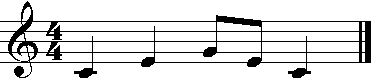
\includegraphics[width=\linewidth]{figures/sonic_pi_comparison.pdf}
        \caption{Notation}
    \end{subfigure}
    \cprotect\caption{A single bar of music represented by the original Sonic Pi syntax, my new metre commands, and traditional Western music notation. Note how the original Sonic Pi syntax loses information about the metre. The second and third arguments to \verb'add_note' are the metrical level and duration.}
    \label{fig:sonicpi_language_comparison}
\end{figure}


\subsection{Metre commands} \label{metre_commands}

A metre is created with the \verb'use_metre' or \verb'with_metre' commands. These have been
designed to match the syntax of existing Sonic Pi commands such as \verb'use_fx' and \verb'with_fx'.

\begin{itemize}
	\item \verb'use_metre(m)' sets the metre to m in the thread local variables
	\item \verb'with_metre(m) do ... end' executes a block of user code with a
specified metre, then restores the original metre
\end{itemize}

The \verb'bar do ... end' command creates a new Bar object, stores this to a
thread local variable, then executes a block of user code. If the Bar object
still has space remaining after the block has run, the function then sleeps for
the appropriate time.


\subsection{Sound commands} \label{sound_commands}

There are three main sound commands: \verb'add_note', \verb'add_sample', and \verb'add_rest'. A
user can use \verb'add_note' to play a note on the current synthesiser. A note is
defined as a pitch (how high or low it sounds) and a duration. The pitch is
specified as in Sonic Pi's \verb'play' command, such as by a note name and octave (C4)
or a MIDI note (60). A list of pitches will sound together as a chord. The
duration is given as a metrical level and a length in units of an event at that
level, as defined in Section~\ref{bar_class}.

The \verb'add_note' command works as follows:
\begin{enumerate}
    \item Gets the current Bar object from the thread local variable store
    \item Calls the Bar's \verb'add_note' method to check if the note will fit into the current bar
    \item Passes the note pitch to Sonic Pi's play function which creates the sound
    \item Sleeps for the duration of the note
\end{enumerate}

I have also implemented some shorthand commands such as \verb'add_quarter' and
\verb'add_whole' which act as wrappers around calls to \verb'add_note'. This was done to
provide an easy-to-use alternative to the metrical level notation for users who
are less familiar with Western music theory. This was especially important as
Sonic Pi was designed to be accessible to primary school children \cite{aaron2013}.

The final two sound commands are \verb'add_sample' and \verb'add_rest'. These function the
same as \verb'add_note' except \verb'add_sample' plays an audio sample and \verb'add_rest' simply sleeps.



\section{Micro-timing} \label{micro-timing_implementation}

In order to add micro-timing functionality to my implementation, I first needed
a way of representing and storing the micro-timing information for different
musical styles. This information is represented by probability distributions for
each event in a metric cycle describing how early or late each event should
occur relative to the metrical grid. In this section, I will describe how the
Style class stores the micro-timing information for a musical style, and how
this is used to apply micro-timing to a user's music.


\subsection{Style class} \label{style_class}

The Style class stores micro-timing values as a Hash from metrical levels (0, 1,
etc.) to lists containing one probability distribution object for each event at
that level. I have implemented a class for a normal distribution, but Style will
accept any distribution object which has a sample method.

The NormalDistribution class is initialised with a mean and standard deviation
and has a method for generating random samples. Samples are generated using the
Box-Muller transform \cite{box1958}, which transforms a pair of uniform random
samples into a pair of normally distributed samples. Sonic Pi's random number
generator is used for the uniform random samples because this generates a
deterministic, repeatable sequence of random numbers, which means the output of
a Sonic Pi program sounds the same each time it is run \cite{aaron2016}.

The class has a test to see if the style is compatible with a given metrical
hierarchy. A Style is defined as being compatible with a MetreTree if, for each
metrical level defined in the Style, it has exactly one distribution for each
metric event at that level in the MetreTree.


\subsection{Applying micro-timing} \label{applying_micro-timing}

When a user sets a metre with the \verb'use_metre' or \verb'with_metre' commands, they can
specify an optional second argument as either a Style object or the name of a
style to be looked up. This causes all music played with that metre to use the
micro-timing of the given style.

At the start of each new bar, the Metre object samples new values from the
Style's probability distributions. When a note is played in the bar, the
\verb'add_note' command requests the timing shift that should be applied to the note
from the Metre. To calculate this, the Metre object calls its
\verb'metrical_level_indices' method (see Section~\ref{metrical_level_indices}) to determine which timing
values from each level to use. These timings are summed to include the
contributions of each metrical level to produce an overall timing shift for the
note. A positive value means the note should be played slightly late; a negative
value means slightly early. This is returned to \verb'add_note' which then uses Sonic Pi's \verb'time_warp' function to adjust the timing of the call to \verb'play'.

For example, if the sampled timings for each level are
\[ T=[0\Rightarrow[0,0.1],1\Rightarrow[0.03,0,0,-0.02]] \]
and the metrical level indices are $L=[0\Rightarrow1,1\Rightarrow3]$, then the timing shift would be calculated as
\[ t=T[0][L[0]]+T[1][L[1]]=0.1+(-0.02)=0.08 \]
Therefore, the note will be played 0.08 quarter lengths late.



\section{Multi-threaded synchronisation} \label{multi-threaded_synchronisation}

An important part of producing music in Sonic Pi is the ability to have multiple
instruments/parts playing simultaneously. This is accomplished by having
separate threads of execution. Aaron et al.'s previous work on Sonic Pi's
temporal semantics [Aaron2014] ensures music in separate threads remains in time.
Because of the probabilistic nature of my implementation of micro-timing, each
thread needs to have the same set of randomly generated timing values to remain
perfectly synchronised. Otherwise, notes in different threads that are supposed
to sound at the same moment might not do so. To tackle this, I implemented a
SynchronisedMetre class which generates new random timing values exactly once
per bar.


\subsection{SynchronisedMetre class} \label{synchronised_metre}

The SynchronisedMetre class is a subclass of Metre which is designed to control
the synchronisation of all the notes contained in the metre. Its main functions,
in addition to those of the Metre class, are:
\begin{itemize}
	\item Set a Style to use for generating micro-timing values
	\item Sample from the Style's probability distributions to get timing values
	\item Compute the total timing shift to be applied to a note at a given offset
	\item Ensure all Bar objects which use it remain synchronised and all have the same set of timing values
\end{itemize}


\subsection{Bar number synchronisation} \label{bar_number_synchronisation}

To make sure Bar objects in separate threads all have the same micro-timing
values, and that these values are regenerated exactly once per cycle, we
synchronise the Bars on the current `bar number'. This is a counter of the
number of bars that have occurred since the beginning of playback. The behaviour
of the Bar class is as follows:

\begin{alltt}
class Bar

    def initialize()
        previous_bar_number = __thread_locals.get(:sonic_pi_bar_number)
        if previous_bar_number
            current_bar_number = @metre.request_bar(previous_bar_number + 1)
        else
            current_bar_number = @metre.request_bar(0)
        end
        __thread_locals.set(:sonic_pi_bar_number, current_bar_number)
    end
end
\end{alltt}

If this is the first bar in the thread, the Bar object will request bar number 0
from the metre, otherwise it will request the next bar number in sequence. The
metre returns the actual current bar number, which is then stored for the next
bar to use.

\begin{alltt}
class SynchronisedMetre < Metre

    def initialize()
        @timings = recalculate_timings()
        @current_bar_number = 0
        @mutex = Mutex.new()
    end

    def request_bar(requested_bar_number)
        @mutex.synchronise do
            if requested_bar_number > @current_bar_number
                @timings = recalculate_timings()
                @current_bar_number = requested_bar_number
            end
        end
        return @current_bar_number
    end
end
\end{alltt}

The SynchronisedMetre's \verb'request_bar' method determines the correct current bar
number. If the requested number is greater than its internal current number,
then it must be the start of a new bar. So, the timings are recalculated, and
its current bar number is updated. If the requested number is old, then it just
returns the current number. The method is synchronised on a mutex to avoid any
race conditions which might cause bars to get different timing values.

\usetikzlibrary{positioning}
\begin{figure}[ht]
    \centering
    \begin{tikzpicture}[node distance=4]
        \node[] (Metre) {SynchronisedMetre};
        \node[right = of Metre] (Thread1) {Thread 1};
        \node[right = of Thread1] (Thread2) {Thread 2};
        \node[below of=Metre, node distance=7cm] (Metre_ground) {};
        \node[below of=Thread1, node distance=7cm] (Thread1_ground) {};
        \node[below of=Thread2, node distance=7cm] (Thread2_ground) {};
        %
        \draw (Metre) -- (Metre_ground);
        \draw (Thread1) -- (Thread1_ground);
        \draw (Thread2) -- (Thread2_ground);
        \draw[->] (Thread1 |- 0,-1) -- node[above,sloped,midway]{requestBar(0)} node[at start,right]{0} node[at end,left]{0} (Metre |- 0,-2);
        \draw[->] (Metre |- 0,-2) -- node[above,sloped,midway]{$b=0$} node[at end,right]{0} (Thread1 |- 0,-2.5);
        \draw[->] (Thread1 |- 0,-3) -- node[above,sloped,midway]{requestBar(1)} node[at end,left]{1} (Metre |- 0,-4);
        \draw[->] (Metre |- 0,-4) -- node[above,sloped,midway]{$b=1$} node[at end,right]{1} (Thread1 |- 0,-4.5);
        \draw[->] (Thread2 |- 0,-5) -- node[above,sloped,midway]{requestBar(0)} node[at start,right]{0} node[at end,left]{1} (Metre |- 0,-6);
        \draw[->] (Metre |- 0,-6) -- node[above,sloped,midway]{$b=1$} node[at end,right]{1} (Thread2 |- 0,-6.5);

    \end{tikzpicture}
    \caption{Sequence diagram demonstrating the behaviour of bar number synchronisation with multiple threads. Values along the vertical axes show that thread's bar number counter. Arrows represent method calls and their return values.}
    \label{fig:multi-threading_sequence_diagram}
\end{figure}

Figure~\ref{fig:multi-threading_sequence_diagram} is a sequence diagram demonstrating the behaviour of the synchronisation
in the presence of multiple threads. Each object/thread's bar number counter is
shown along its axis. Each thread's counter is initialised to 0. Thread 1
requests bar 0, which is equal to the SynchronisedMetre's current value, so $b=0$
is returned. Thread 1 then requests the next bar number (1). This is greater
than the SynchronisedMetre's current value, so its value is updated and returned.
Thread 2 then starts late and requests an old bar number (0). The
SynchronisedMetre recognises this is old, so simply returns its current value
$b=1$ so Thread 2 can catch up.



\section{Jembe data analysis} \label{jembe_data_analysis}

Creating music with realistic micro-timing using the implementation I have
described requires a set of probability distributions which accurately
characterise a style of music. Therefore, these distributions must be derived
from real-life examples of music. The next two sections describe the data
collection and analysis that was done for the jembe and Viennese waltz styles.
The results of the data analysis methods described here can be found in
SUBSECTION.


\subsection{Datasets} \label{jembe_datasets}

Previous research into the micro-timing of Malian jembe music has meant there
are some high-quality datasets of processed live recordings available.

The first dataset is from Jacoby et al. [Jacoby2021] and consists of 11
processed recordings of a piece called `Suku', which is a very commonly played
piece in this style. The recordings were made by Rainer Polak in Bamako, Mali in
2016 [Jacoby2021supp].

The second dataset is from the Interpersonal Entrainment in Music Performance
(IEMP) Data Collection [Polak2018][Clayton2021]. This consists of 15 recordings
across three different pieces: `Manjanin', `Maraka', and `Woloso'. The
recordings were again made by Polak in Bamako in 2006 and 2007. See APPENDIX for
a full list of performers.

The datasets supply the following data:
\begin{itemize}
	\item Onset time -- the time when a drum stroke occurs
	\item Cycle number
	\item Metric location -- which metric event the onset belongs to
	\item Phase -- the actual timing of the onset within the cycle
\end{itemize}


\subsection{Micro-timing estimation} \label{jembe_micro-timing}

The pieces of jembe music in the dataset use a metre with four beats, each of
which divides into three, for a total of 12 metric events at the first division
level (often notated as \setmetre{12}{8}). It is at this level, referred to as the `pulse', that the micro-timing occurs.

Each event at the pulse level has a position in the cycle at which a note would
occur if it were isochronous. The offset from this position describes the
micro-timing of a note, and this is what is stored in the probability
distributions described in SUBSECTION. Equation~\ref{eq:offset_from_phase} shows how the offset is calculated from the phase given by the datasets.

\begin{equation}
    \textnormal{offset} = \frac{(\textnormal{phase} \times \textnormal{beat division}) - \textnormal{metric location}}{2}
    \label{eq:offset_from_phase}
\end{equation}

The phase is multiplied by the beat division (in this case, 3) to convert it
into pulse units. The metric location at the pulse level (integer from 0 to 11)
is subtracted to get the offset. The final division by two converts the offset
into quarter lengths (because each pulse unit is an eighth length).

Once the offset has been calculated for each drum stroke, I was then able to
estimate the distribution of offsets for each of the twelve metric locations. I
considered two types of approach for probability density estimation:

\begin{itemize}
	\item Kernel density estimation (non-parametric) -- applies smoothing to the
data to fit an arbitrary distribution
	\item Maximum likelihood estimation (parametric) -- choose an existing
distribution to fit and estimate the parameters which fit the data the best
\end{itemize}

The advantage of KDE is that it would be able to accurately represent any shape
of distribution the data may have. However, it stores each point which describes
the probability density function. This means it generally has a higher memory
requirement than MLE which only stores the values of the parameters. Another
advantage of MLE is it allows hypothetical distributions to be easily defined
without the need for data.

For this scenario, I chose to use MLE to fit a normal distribution to the data.
A normal distribution was suitable because the data was assumed to be estimating
a theoretical true value of the offset. A normal distribution requires two
parameters: the mean, $\mu$, and the standard deviation, $\sigma$. It can be shown that the
maximum likelihood estimator for the population mean $\hat{\mu}$ is the sample mean $\bar{x}$,
and the estimator for the population standard deviation $\hat{\sigma}$ is the sample
standard deviation $s$ [Dekking2005]. The calculation of $s$ uses Bessel's
correction to get an unbiased estimator of $\hat{\sigma}$ [Upton2008].


\subsection{Tempo estimation} \label{tempo_estimation}

Generating a synthetic piece of jembe music requires analysis of other musical
features as well as the micro-timing to sound realistic. One of these is the
tempo (how fast or slow the beat is), which is measured in beats per minute
(bpm). The tempo of a jembe piece of music typically increases substantially
over the duration of the performance [Jacoby2021], with the last 15 seconds or
so showing the tempo increasing at a much faster rate.

The inter-beat interval is defined as the time between two subsequent beats in a
piece of music from which the instantaneous tempo can be calculated [Dixon2002].
A moving average can be applied to the instantaneous tempo to obtain an estimate
of the global tempo.

For the jembe data, I first filtered all the onsets to include just those played
by Jembe 2 (because it plays on each beat) [Jacoby2021], then filtered these to
just onsets on the beats. I then calculated the inter-beat interval using Equation~\ref{eq:ibi}, where $b_i$ is the onset time of the $i$th beat. This is then converted to bpm by Equation~\ref{eq:tempo}. A moving average with window size 10 is then applied to smooth the tempo.

\begin{equation}
    \mathrm{IBI}_i = b_i - b_{i-1}
    \label{eq:ibi}
\end{equation}
\begin{equation}
    t_i = \frac{60}{\mathrm{IBI}_i}
    \label{eq:tempo}
\end{equation}

Inspection of the smoothed tempo graphs showed a logarithmic trend for the first $\sim95\%$ of the piece. A sharper increase follows this which was
modelled by a quadratic curve. To fit curves to the data, I used the \verb'optimize.curve_fit' function from the SciPy Python library, which uses non-linear least
squares. The parameters estimated by the curve fitting are then used in Sonic Pi
to control the tempo of a synthetic jembe piece during playback.


\subsection{Rhythm patterns} \label{rhythm_patterns}

The final data analysis performed on the jembe music was an analysis of the
rhythm patterns played by Jembe 1. While the other instruments in the ensemble
play repetitive accompaniments, Jembe 1 has a lead role and can play a variety
of rhythmic patterns, also often involving improvisation. By analysing these
patterns, I was able to produce a synthetic Jembe 1 part for Suku with
semi-realistic rhythms. My approach was as follows:

\begin{enumerate}
    \item Compute the rhythm played by Jembe 1 in each cycle as a 12-bit binary number, where the bit value at each position indicates whether there was an onset at the corresponding pulse in that cycle
    \item Convert the 12-bit binary numbers into a decimal integer for each cycle
    \item Count the number of times rhythm $x$ is followed by rhythm $y$ and calculate transition probabilities from these
    \item Generate a random sequence of rhythm integers using the transition probabilities
    \item During playback, for each cycle, play a drum stroke on pulse $i$ if there is a 1 at bit $i$ in the binary representation of that cycle's rhythm integer
\end{enumerate}

This approach was an improvement over purely random rhythms because it preserved
intra-cycle patterns. The jembe can be played with three different techniques,
each producing a different kind of sound (timbre). These are tone, slap, and
bass. To include this, I created a roughly typical pattern covering each note
position in the cycle: [T,T,S,T,T,S,B,B,S,B,B,S]. If a note is played at a
particular pulse, the corresponding timbre is looked up from this pattern.



\section{Waltz data analysis} \label{waltz_data_analysis}

The Viennese waltz provides a useful comparison to Malian jembe in evaluating
this project's micro-timing implementation. This style uses a metre with three
beats (\setmetre{3}{4}) and the micro-timing can be observed at the beat level, where the
second beat is usually early. The micro-timing in Viennese waltz has not been
studied in as much detail or as recently as jembe, so there were no existing
datasets of Viennese waltz performances with micro-timing. This meant further
calculations were needed to derive it, which will be explained in this section.


\subsection{Datasets} \label{waltz_datasets}

I first considered using the Ballroom dataset [Gouyon2006], which contains
30-second recordings of 65 pieces of Viennese walt music, and for which
annotations of the beats exists [Krebs2013]. However, when I listened to the
recordings, I didn't notice any micro-timing. To test my suspicions, I performed
the micro-timing analysis described in SUBSECTION and then conducted a
one-sample t-test. This tests whether the sample mean of the offset of the
second beat is statistically significantly different from 0 (the case where
there is no micro-timing). At the 5\% significance level, there were very few
recordings which had any significant micro-timing, so this dataset was deemed
unsuitable. See SUBSECTION for the full results of the test.

I then constructed my own dataset comprising of 30-second samples from seven
waltz recordings performed by the Vienna Philharmonic Orchestra, all of which
have noticeable and statistically significant micro-timing. Because this dataset
has no existing beat annotations, this step needed to be performed next.


\subsection{Beat tracking} \label{beat_tracking}

Beat tracking is the process of identifying the locations of beats in an audio
recording of a piece of music. Since the beat level is where the micro-timing in
the Viennese waltz occurs, no additional onset detection was necessary. The beat
tracking could be approached automatically with existing beat tracking
algorithms, or manually.

A variety of automatic beat tracking algorithms were tried, but most didn't
perform well. Many implementations struggled because they expect the beats to be
isochronous, i.e.\ having no systematic micro-timing, as is the case in most
Western music. As a result, they would often skew the detected beats towards
being isochronous, therefore not capturing the micro-timing. Of all these
implementations, the beat tracking in the libfmp Python library [Mueller2021] (a
dynamic programming approach from Müller's Fundamentals of Music Processing
[Mueller2021b]) performed the best (see SUBSECTION for results). After some
small manual corrections, the beat onsets were ready for analysis, as described
in SUBSECTION.

As an alternative, manual beat annotations were created using the Sonic
Visualiser software [Cannam2010]. While the micro-timing from this approach was
more prominent, the data had a large variance which led to the generated music
sounding erratic. For this reason, the automatic approach was chosen.


\subsection{Micro-timing estimation} \label{waltz_micro-timing}

To calculate the micro-timing offset of each beat from just the onset time
involves first identifying the start and end of each cycle, estimating the onset
of each beat if they were isochronous, then finding the difference between this
and the actual onset to get the offset. The full calculation is shown in
Equation~\ref{eq:offset_from_onset}, where $i$ ranges over the indices of all the onsets in the piece.

\begin{equation}
\begin{split}
    \mathrm{metricLocation}_i &= i \;\mathrm{mod}\; 3 \\
    \mathrm{cycleStart}_i     &= \mathrm{onset}_{i-\mathrm{metricLocation}_i} \\
    \mathrm{cycleEnd}_i       &= \mathrm{onset}_{i-\mathrm{metricLocation}_i+3} \\
    \mathrm{cycleDuration}_i  &= \mathrm{cycleEnd}_i - \mathrm{cycleStart}_i \\
    \mathrm{isochronousBeatDuration}_i &= \frac{\mathrm{cycleDuration}_i}{3} \\
    \mathrm{isochronousOnset}_i &= \mathrm{cycleStart}_i + (\mathrm{metricLocation}_i \times \mathrm{isochronousBeatDuration}_i) \\
    \mathrm{offset}_i &= \frac{\mathrm{onset}_i-\mathrm{isochronousOnset}_i}{\mathrm{isochronousBeatDuration}_i} \\
    \mathrm{phase}_i          &= \mathrm{offset}_i + \mathrm{metricLocation}_i
\end{split}
\label{eq:offset_from_onset}
\end{equation}

The data is assumed to have exactly one onset for each beat in the piece and the
duration of a cycle is assumed to be the time between its first beat and the
first beat of the next cycle.

Once the offsets have been derived, maximum
likelihood estimation is used to get the distributions, as described in
SUBSECTION.



\section{MusicXML converters} \label{musicxml_converters}

MusicXML is a commonly used file format for encoding Western music notation
which is based on XML. In preparation for the evaluation, I have also
implemented a pair of converter programs between MusicXML and my extended Sonic
Pi language.

\begin{itemize}
	\item \verb'convert_mxl.py' uses the \verb'music21' Python library to parse an input MusicXML file into Python objects, which are then iterated over to produce Sonic Pi code
	\item \verb'convert_sonicpi.rb' takes an input Sonic Pi file and iterates over it to produce \verb'music21' Python code. This code is then run automatically which generates the final MusicXML output
\end{itemize}

The most interesting part of the converters is the \verb'convert_duration' algorithm
which converts a note specified by its quarter length duration into a (metrical
level, multiplier) pair. This is essentially the inverse of the Bar class's
\verb'add_note' method, which converts a metrical level and multiplier into a quarter length duration (see Section~\ref{bar_class}).

The algorithm first tries to find a metrical
level whose value the note's duration divides into. For example, if the metre
has levels made up of durations $\left[\frac{1}{4},\frac{1}{8},\frac{1}{16}\right]$, then a note with duration $\frac{5}{16}$
can only exist at the third level, so the algorithm would return $(3,5)$.

If no
such level can be found, then deeper metrical levels must be searched, where we
assume they are divided into two each time. The note's duration in quarter
lengths is first converted to a fraction by dividing by 4. The level $l$ and
multiplier $m$ can then be found as in Equation~\ref{eq:duration_to_level_multiplier}, where $\log_2\left(\frac{n_d}{\mathrm{deepestDenominator}}\right)$ is the number of levels deeper we need to
go.

\begin{equation}
    \begin{split}
        \frac{n_n}{n_d} &= \frac{\mathrm{duration}}{4} \\
        l &= \left\lfloor \mathrm{deepestLevel} + \log_2\left(\frac{n_d}{\mathrm{deepestDenominator}}\right) - 1 \right\rfloor  \\
        m &= n_n
    \end{split}
    \label{eq:duration_to_level_multiplier}
\end{equation}





\chapter{Evaluation} \label{evaluation}

Text.



\chapter{Conclusions} \label{conclusions}

Text.




\printbibliography[title=References]

\end{document}
